\section{Tutorial}
Let's see in practice what we have previously learnt in a simple tutorial: first of all, we need the whole program, available at \textit{ https://github.com/BFSteam/memory.}
Once we put it in the same folder containing SLAPP3, we need to connect the two programs inserting memory \textbackslash src path in SLAPP3 \textbackslash project.txt as described in \textit{SLAPP\_Reference\_Handbook.pdf pag20}.
Now, inside SLAPP3, we can run the program runShell.py, for example by terminal.
At the very beginning, we confirm \textit{memory} path and project. Then, we have to set all the necessary input variables to start the simulation:
\begin{itemize}
\item[\texttt{Random number seed:}] insert the seed to provide the entire reproducibility of a single simulation.
\item[\texttt{Number of sources:}]insert the number of sources inside the network.
\item[\texttt{Number of users:}]insert the number of users inside the network.
\item[\texttt{Average degree for users:}]insert the value of the average degree for users only.
\item[\texttt{Number of cycles:}]insert the maximum number time can reaches.
\end{itemize}

In order to simplify our first approach, default values are provided to all previous variables by pressing Enter, and that's it!
Simulation is running and our network is evolving. A window will appear with the drawing network\footnote{The runtime network is drawn using the libraries networkx and matplotlib.} and in terminal the flowing time is displayed. 
Nodes of the network are painted with different colours: if they don't spread, grey for inactive state and blue for active one; if they spread, they can be orange, pink or cyan depending on the spreaded news. In detail, every source initially generates a single news, tracked by its colour. Sources are bigger than users and labeled with 0,1 and 2; numbering goes on with users.\\
\begin{figure}
  \centering
  \begin{subfigure}[t]{.45\textwidth}
    \centering
    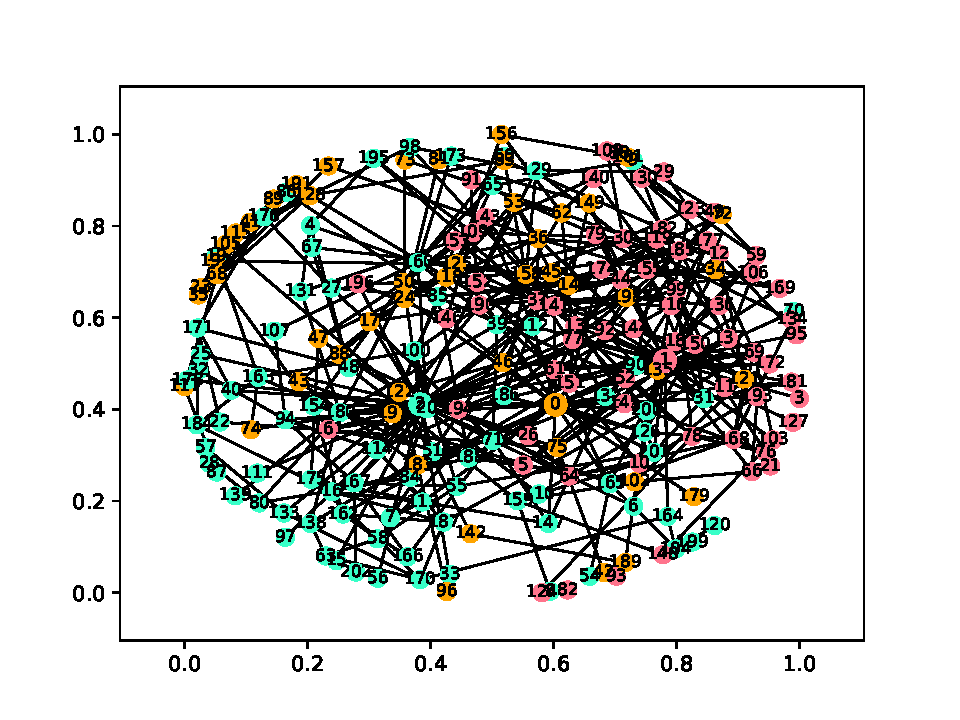
\includegraphics[trim={1cm .5cm 1cm 1cm}, clip, width=\linewidth]{img/pdf/plot-0100.pdf} 
    \caption{100 cycles} \label{fig:100}
  \end{subfigure}
  \begin{subfigure}[t]{.45\textwidth}
    \centering
    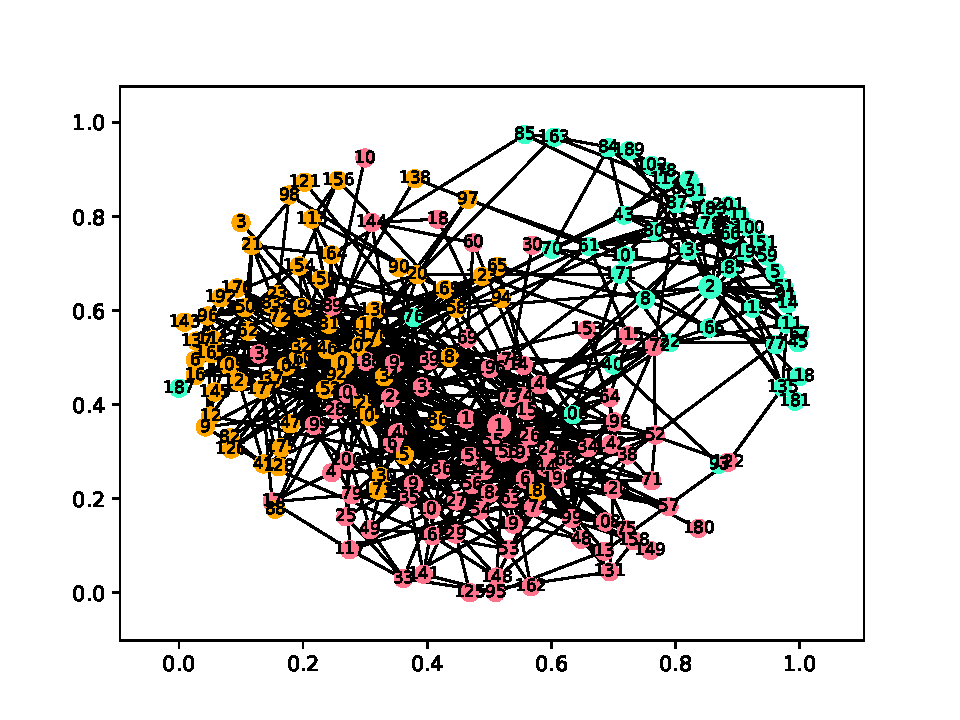
\includegraphics[trim={1cm .5cm 1cm 1cm}, clip, width=\linewidth]{img/pdf/plot-0200.pdf} 
    \caption{200 cycles} \label{fig:200}
  \end{subfigure}

  \vspace{0cm}

  \begin{subfigure}[t]{.45\textwidth}
    \centering
    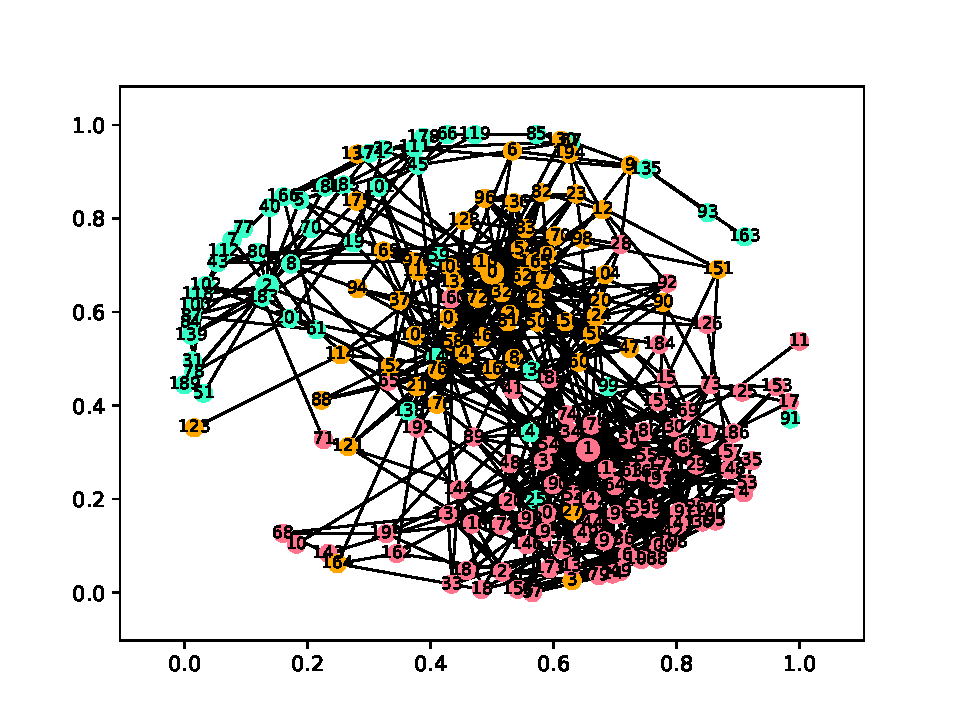
\includegraphics[trim={1cm .5cm 1cm 1cm}, clip, width=\linewidth]{img/pdf/plot-0300.pdf} 
    \caption{300 cycles} \label{fig:300}
  \end{subfigure}
  \begin{subfigure}[t]{.45\textwidth}
    \centering
    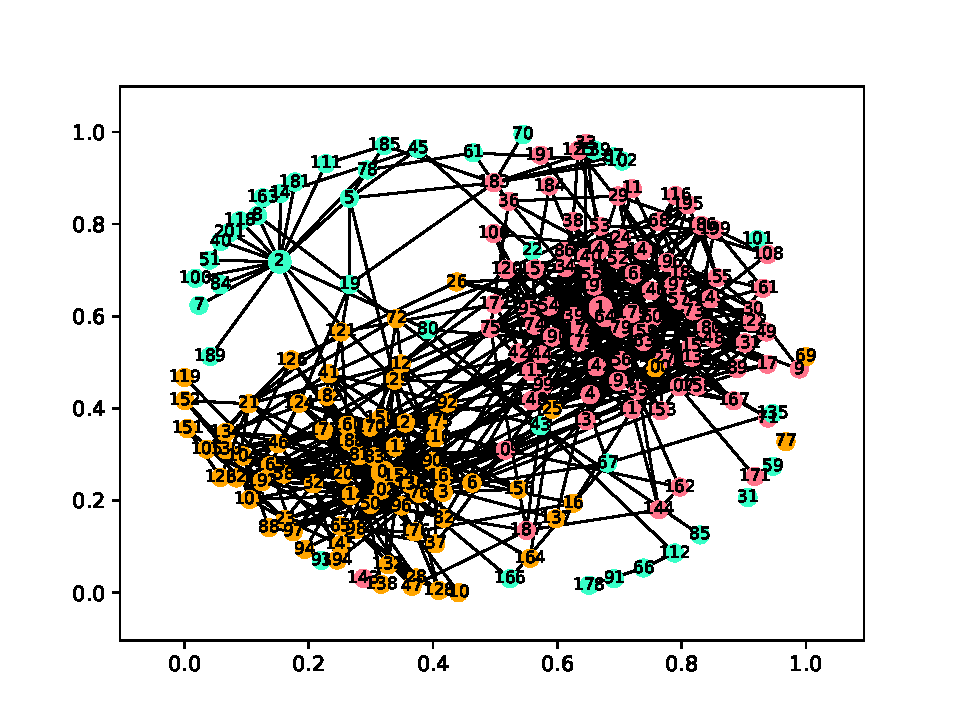
\includegraphics[trim={1cm .5cm 1cm 1cm}, clip, width=\linewidth]{img/pdf/plot-0400.pdf} 
    \caption{400 cycles} \label{fig:400}
  \end{subfigure}

  \begin{subfigure}[t]{.45\textwidth}
    \centering
    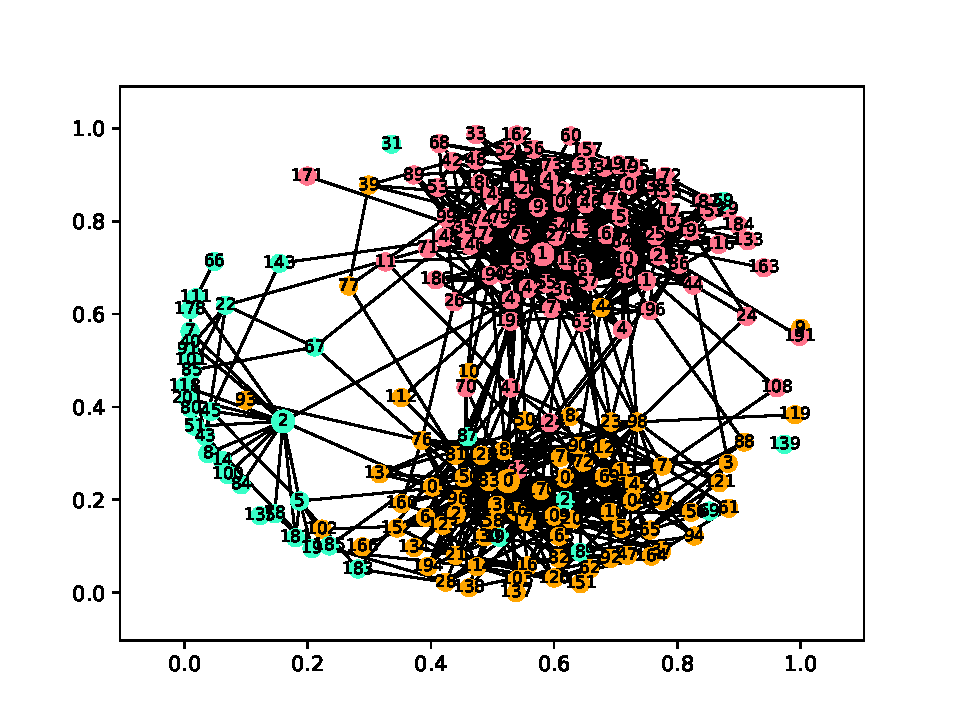
\includegraphics[trim={1cm .5cm 1cm 1cm}, clip, width=\linewidth]{img/pdf/plot-0500.pdf} 
    \caption{500 cycles} \label{fig:500}
  \end{subfigure}
  \begin{subfigure}[t]{.45\textwidth}
    \centering
    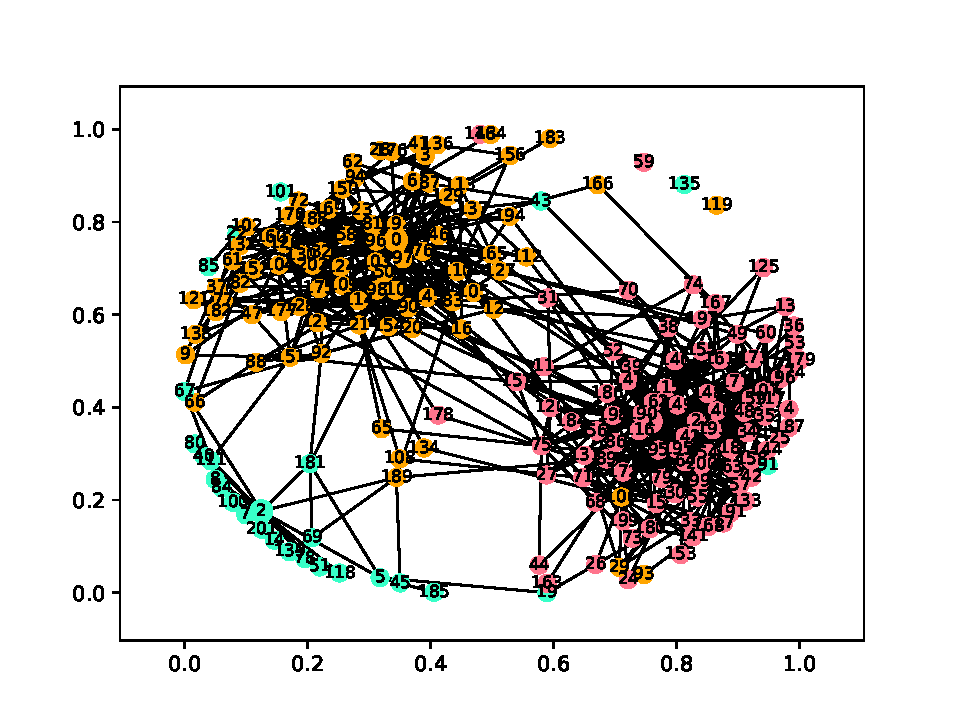
\includegraphics[trim={1cm .5cm 1cm 1cm}, clip, width=\linewidth]{img/pdf/plot-0600.pdf} 
    \caption{600 cycles} \label{fig:600}
  \end{subfigure}
  
  \caption{Plot at different time steps for a simulation with 3 sources, 200 users, initial average degree of users 5 and 600 timesteps. Random seed initialized to 123456789}
\end{figure}

- common var
-schedule
-observerActions.txt
networkx
